\chapter{Filters II}

\section{More on convolution}
\begin{itemize}
    \item \textbf{Convolution}: $(f * h)[n,m] = \sum_{k,l}f[k,l] h[n-k, m-l]$
    \item \textbf{Cross-correlation}: $(f$ \ding{72} $h)[n,m] = \sum_{k,l}f[k,l] h[n+k, m+l]$
\end{itemize}
The only difference between the two is the way the kernel is applied. In fact, a convolutive operator applies a flipped version, in both dimension, of the sliding window.
\begin{center}
    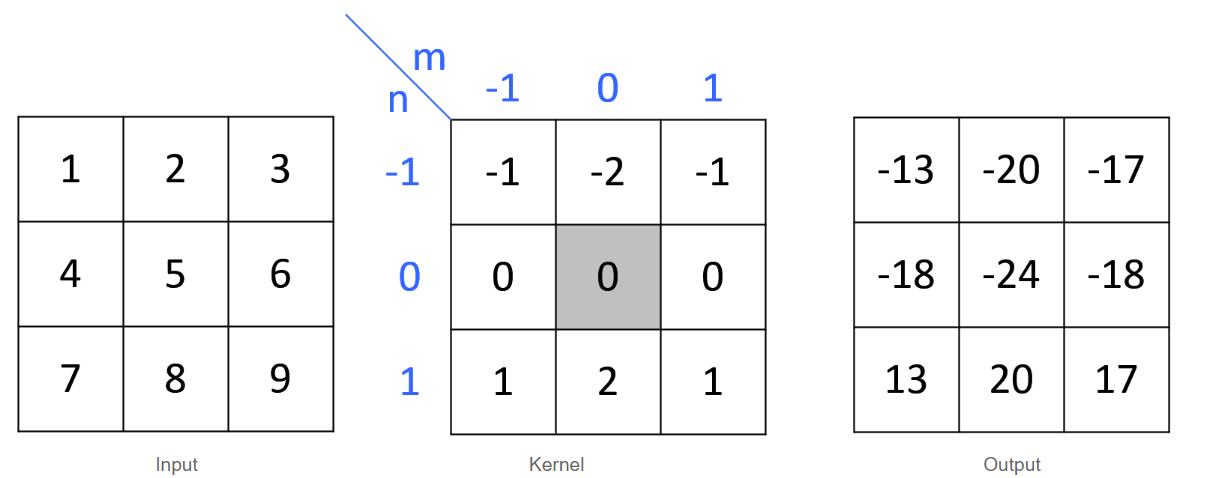
\includegraphics[scale =0.5]{images/flipped kernel.png}
\end{center}
more details here: \url{ http://www.songho.ca/dsp/convolution/convolution2d_example.html}

\subsection{Properties of convolution}
\begin{itemize}
    \item \textbf{Commutative}: $(f * g) = (g * f)$
    \item \textbf{Associative}: $(f * g) * h = f * (g * h)$
    \item \textbf{Homogeneity}: $\textbf{k}f*g = f*\textbf{k}g = \textbf{k}(f*g)$
    \item \textbf{Distributive}: $f * (g + h) = (f * g) + (f * h)$
    \item \textbf{Shift invariant}: Operator behaves the same everywhere, i.e. the value of the output depends on the pattern in the image neighborhood, not on the position of the neighborhood
    \item \textbf{Separability}: 2D convolution is separable, and we can factor into two steps (i.e. first convolve all rows with a 1D filter, then convolve all columns with a 1D filter).
\end{itemize}

\section{Sharpening filters}
A sharpening filter emphasizes image details. They are high pass filters that emphasize high frequencies, and penalize low frequencies.\newline
The sharpening effect is obtained in two steps:
\begin{itemize}
    \item Apply an operator that extracts the details of the image (produces an image with light values in the transition areas and dark values in the uniform areas)
    \item This result is added to the original image
\end{itemize}
One way to obtain the details is by applying a smoothing filter to an image and computing a pixel by pixel difference between the original image and the smoothed one. Then you add the resulting image to the original one to obtain the sharpening effect.
\begin{flushleft}
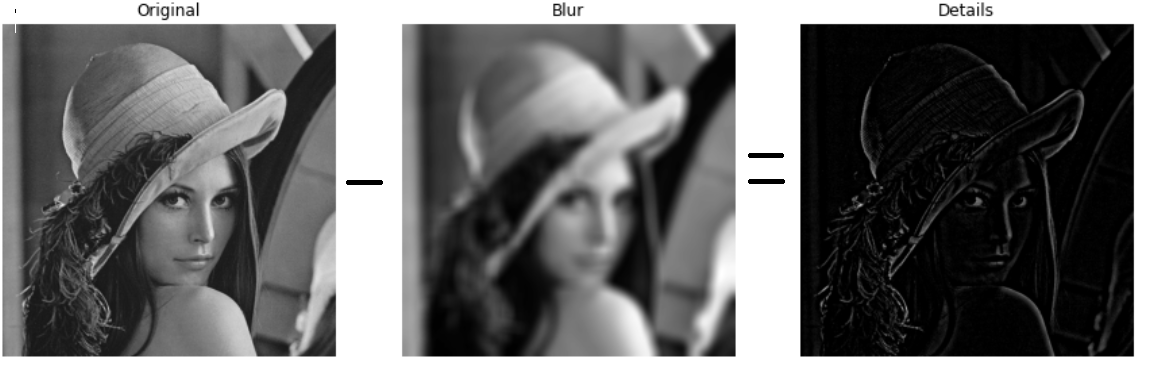
\includegraphics[scale=0.6]{images/details.png}
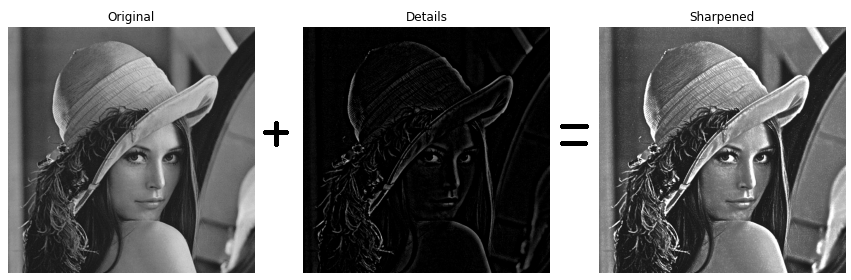
\includegraphics[scale = 0.8]{images/Lena sharpened.png}
\end{flushleft}
\section{Edge detection}
An edge is a set of connected pixels between two regions in which there is a sudden change in intensity. These discontinuities can be caused by:
\begin{itemize}
    \item Illumination discontinuity: cast shadows
    \item Change in surface orientation: shape
    \item Depth discontinuity: object boundary
    \item Surface color discontinuity
\end{itemize}
The goal of edge detection is to detect easily and automatically these regions.\newline
Basically, a simple edge detection algorithm computes the first order derivative of the intensity function of an image and detects as edges the extremes of the derivative function.
\begin{flushleft}
    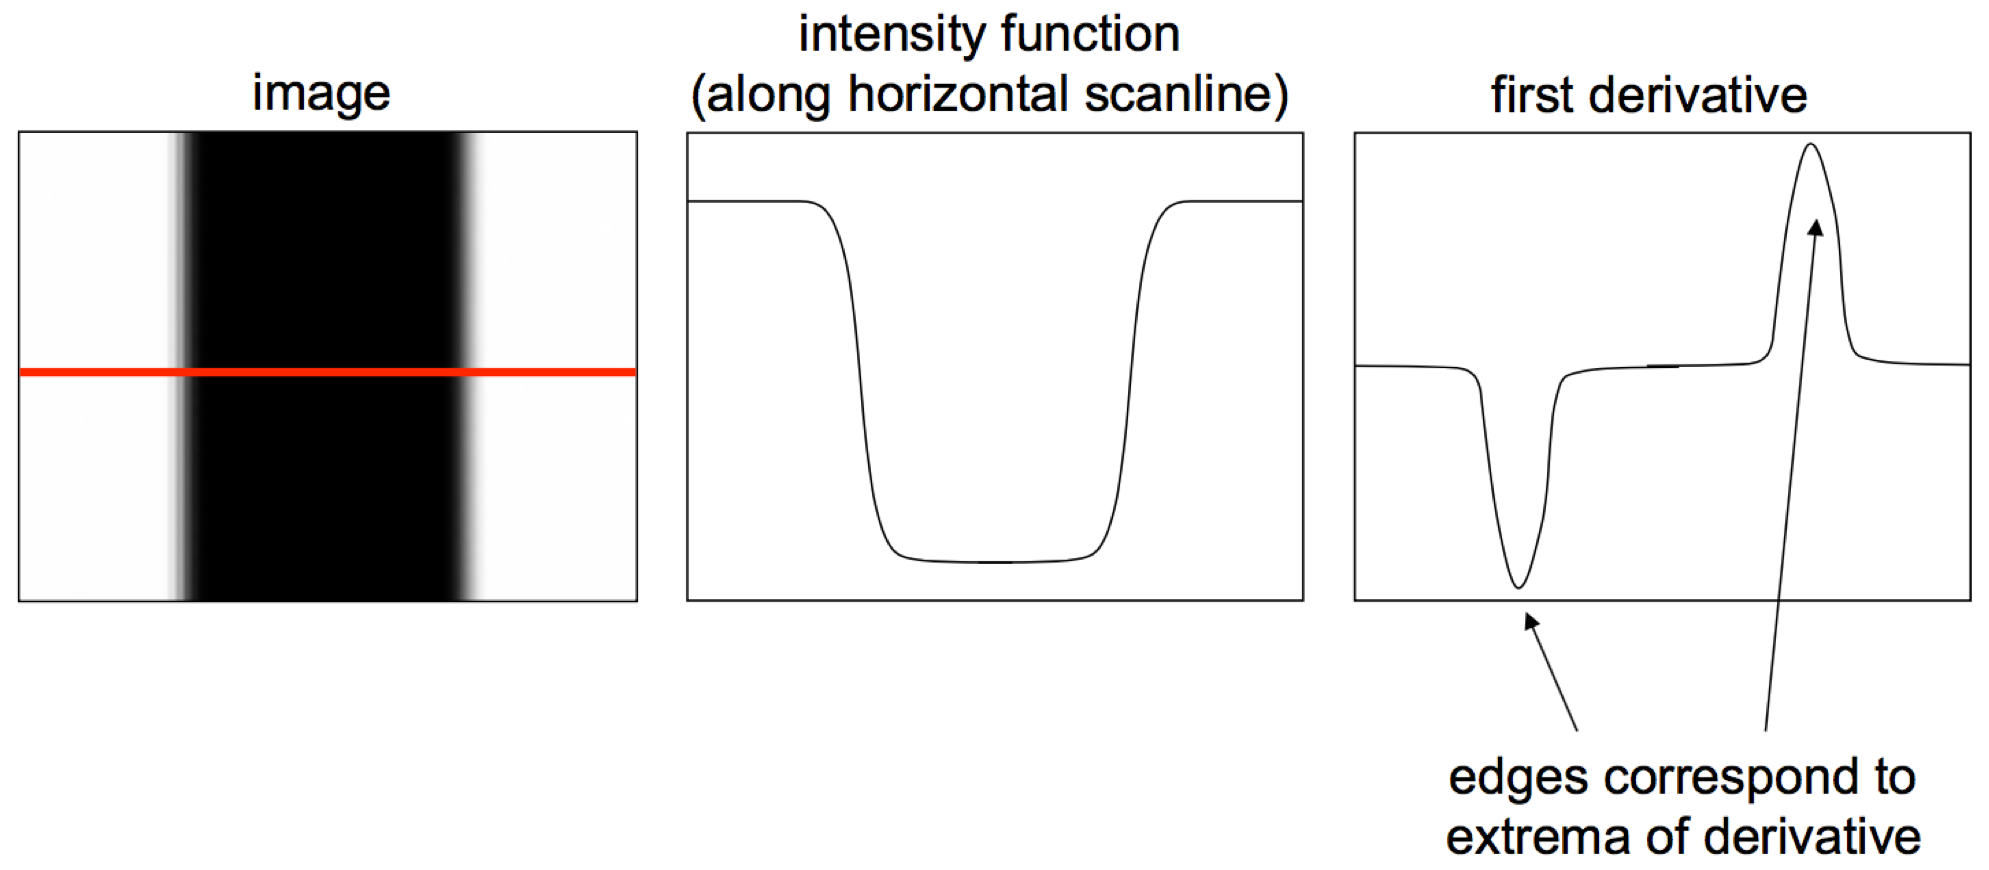
\includegraphics[scale = 0.4]{images/edge detection.png}
\end{flushleft}
\subsection{Discrete approximation of the derivatives}
In order to apply a derivative operator in a digital environment, we need a discrete approximation of derivatives. 
\begin{itemize}
    \item Derivative in 1D:
    \[\frac{df}{dx} = lim_{\Delta x \rightarrow 0} \frac{f(x) - f(x - \Delta x)}{\Delta x} = f^{'}(x)\]
    \item Discrete derivative in 1D:
    \[\frac{df}{dx} = lim_{\Delta x \rightarrow 0} \frac{f(x) - f(x - \Delta x)}{\Delta x} = f^{'}(x)\]
    \[= \frac{f(x) - f(x - 1)}{1} = f^{'}(x)\]
    \[= f(x) - f(x - 1) = f^{'}(x)\]
\end{itemize}
Operators based on the first order derivative must satisfy the following properties:
\begin{itemize}
    \item have zero value in the homogeneous sections of the image (no response in constant regions)
    \item have a non-zero value along the transition areas.
\end{itemize}
Formulations satisfying these properties can be defined in terms of differences between pixel values.
\begin{flushleft}
    \begin{tabular}{c | c | c}
     \textbf{Name} & \textbf{Discrete derivative} & \textbf{Filter}\\
     \hline\xrowht{20pt}
     Backward & $\frac{df}{dx} = f(x) - f(x-1)$ & [0 1 -1]  \\
     \xrowht{20pt}
     Forward & $\frac{df}{dx} = f(x) - f(x+1)$ & [-1 1 0]\\
     \xrowht{20pt}
     Central & $\frac{df}{dx} = f(x+1) - f(x-1)$ & [1 0 -1]
    \end{tabular}
\end{flushleft}
Note that each discrete approximation can be defined as an application of convolution using the respective 1D filter (the same is valid also for 2D images).\newline\newline\newline\newline\newline\newline
\textbf{Backward example:}
Backward derivative is obtained by computing the difference between the value of the current pixel and the value of the previous one.
\begin{flushleft}
    \begin{tikzpicture}
    \matrix[matrix of nodes, row 1 column 1/.style={nodes={draw=none, fill=none}},nodes={minimum size=0.5cm, draw}, row sep=-\pgflinewidth, column sep=-\pgflinewidth](mygrid){%
    $f(x) = $ & 10 & 15 & 10 & 10 & 25 & 20 & 20 & 20\\
    };
    \end{tikzpicture}
    
    \begin{tikzpicture}
    \matrix[matrix of nodes, row 1 column 1/.style={nodes={draw=none, fill=none}},nodes={minimum size=0.5cm, draw}, row sep=-\pgflinewidth, column sep=-\pgflinewidth](mygrid2){%
    $f^{'}(x) = $ & 0 & 5 & -5 & 0 & 15 & -5 & 0 & 0\\
    };
    \end{tikzpicture}
\end{flushleft}
That is the same of applying convolution using the kernel [0 1 -1] (flipped).\newline \newline
According to this, a 2D derivative filter could be defined by the following kernels (central derivative):
\begin{figure}[h]
        \centering
        \begin{minipage}{0.45\linewidth}
        \centering
        \begin{tikzpicture}
            \matrix[matrix of nodes ,nodes={minimum size=0.5cm, draw}, row sep=-\pgflinewidth, column sep=-\pgflinewidth](sobel_hz){%
            1 & 1 & 1\\
            0 & 0 & 0\\
            -1 & -1 & -1\\
            };
        \end{tikzpicture}
        \caption*{Detects horizontal edges}
        \end{minipage}
        \hspace{20pt}
        \begin{minipage}{0.45\linewidth}
        \centering
        \begin{tikzpicture}
            \matrix[matrix of nodes ,nodes={minimum size=0.5cm, draw}, row sep=-\pgflinewidth, column sep=-\pgflinewidth](sobel_v){%
            1 & 0 & -1\\
            1 & 0 & -1\\
            1 & 0 & -1\\
            };
        \end{tikzpicture} 
        \caption*{Detects vertical edges}
        \end{minipage}
\end{figure}

\subsection{Image gradient}
The operators based on the first order derivative are formulated starting from \textbf{gradient}. Given a function $f(x,y)$ (2D image), the gradient vector is defined as follows:
\[
    \nabla f = 
    \begin{bmatrix}
        G_{x}\\
        G_{y}\\
    \end{bmatrix}
    =
    \begin{bmatrix}
        \frac{\partial f}{\partial x}\\
        \vspace{1pt}\\
        \frac{\partial f}{\partial y}\\
    \end{bmatrix}
\]
The image gradient is obtained by applying two-dimensional derivative filters and it provides the following information:
\begin{itemize}
    \item The partial derivatives with respect to both horizontal and vertical directions.
    \item The gradient magnitude, which indicates the intensity of the discontinuity.
    \[|| \nabla f || = \sqrt{G_{x}^{2} + G_{y}^{2}}\]
    \item The gradient direction, given by:
    \[ \theta = tan^{-1} \left (\frac{G_{y}}{G_{x}} \right)\]
    \item It points in the direction of most rapid increase in intensity.
\end{itemize}
\begin{center}
    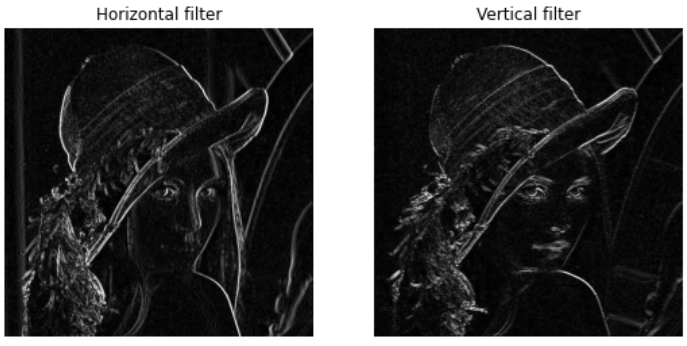
\includegraphics[scale = 0.8]{images/lena hx hy.png}
\end{center}
\subsection{Effects of noise}
Derivative operators are sensitive to noise. Thus, it may be impossible to detect edges of a noisy image (even if the noise is not so strong).
In these cases it is useful to perform a smoothing operation before applying the derivative filter.\newline
For example, we can look for peaks in $\frac{d}{dx}(f * g)$ where $g$ is a smoothing kernel (e.g. Gaussian filter). By applying the differential property of convolution
\[\frac{d}{dx}(f * g) = f * \frac{d}{dx}g\]
which save us one operation. In fact, by doing this, you obtain a new filter $ \frac{d}{dx}g$ called \textbf{derivative of Gaussian} that performs at the same time both smoothing and derivative operation
